\documentclass{standalone}
\usepackage{pgf,tikz}
\usetikzlibrary{decorations.pathreplacing}

\begin{document}
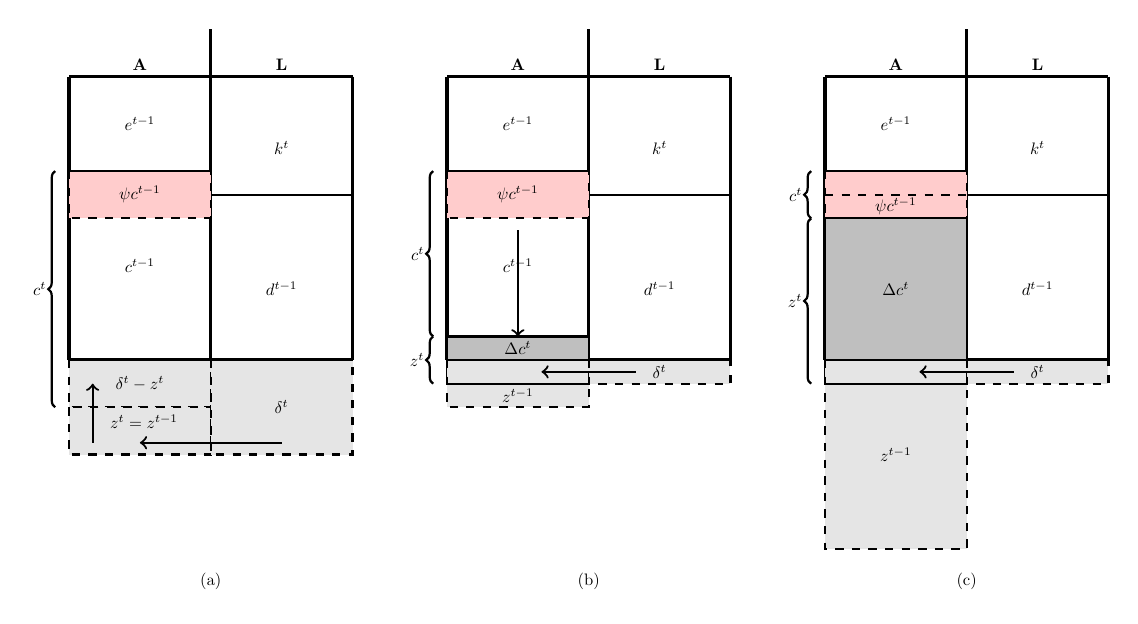
\begin{tikzpicture}[thick,scale=0.6, every node/.style={scale=0.6}]

%%%%%%%%%%%%%%%%%%%%%% CASE I %%%%%%%%%%%%%%%%%%%%%%

% Border and preliminaries
\draw [very thick] (0, 6) to (6, 6);
\draw [very thick] (6, 6) to (6, 0);
\draw [very thick] (6, 0) to (0, 0);
\draw [very thick] (0, 0) to (0, 6);

\draw [very thick] (3, 7) to (3, 0);
    \node [above] at (1.5, 6) {\textbf{A}};
    \node [above] at (4.5, 6) {\textbf{L}};
    
\node [above] at (3, -5) {(a)};
    
% Initial balance sheet  
%Assets
\node at (1.5, 5) {$e^{t-1}$};
\node at (1.5, 2) {$c^{t-1}$};
\draw [fill=red!20,dashed] (0,4) rectangle (3,3);
    \node  at (1.5,3.5) {$\psi c^{t-1}$};
    \draw [thick] (0,4) to (3,4);
%Liabilities
\node at (4.5, 4.5) {$k^{t}$};
    \draw [thick] (3,3.5) to (6,3.5);
\node at (4.5, 1.5) {$d^{t-1}$};

% After deposit shock and adjustment

%Assets
\draw [fill=gray!20,dashed] (0,0) rectangle (3,-1);
    \node  at (1.5,- 0.5) {$\delta^{t}-z^{t}$};
\draw [fill=gray!20,dashed] (0,-1) rectangle (3,-2);
    \node  at (1.5,- 1.3) {$\,\,\,z^{t}=z^{t-1}$};
    
\draw[decoration={brace,raise=5pt},decorate]
    (0,-1) -- node[left=10pt] {$c^{t}$} (0,4);
    
%Liabilities
\draw [fill=gray!20,dashed] (3,0) rectangle (6,-2);
    \node  at (4.5,- 1) {$\delta^{t}$};
  
\draw[thick,->] (4.5,-1.75) to (1.5,-1.75);
\draw[thick,->] (0.5,-1.75) to (0.5,-0.5);
    
%%%%%%%%%%%%%%%%%%%%%% CASE II-1 %%%%%%%%%%%%%%%%%%%%%%

% Border and preliminaries
\draw [very thick] (8, 6) to (14, 6);
\draw [very thick] (14, 6) to (14, 0);
\draw [very thick] (14, 0) to (8, 0);
\draw [very thick] (8, 0) to (8, 6);

\draw [very thick] (11, 7) to (11, 0);
    \node [above] at (9.5, 6) {\textbf{A}};
    \node [above] at (12.5, 6) {\textbf{L}};
    
\node [above] at (11, -5) {(b)};

% Initial balance sheet  
%Assets
\node at (9.5, 5) {$e^{t-1}$};
\node at (9.5, 2) {$c^{t-1}$};
\draw [fill=red!20,dashed] (8,4) rectangle (11,3);
    \node  at (9.5,3.5) {$\psi c^{t-1}$};
    \draw [thick] (8,4) to (11,4);
%Liabilities
\node at (12.5, 4.5) {$k^{t}$};
    \draw [thick] (11,3.5) to (14,3.5);
\node at (12.5, 1.5) {$d^{t-1}$};

% After deposit shock and adjustment

%Assets
\draw [fill=gray!50] (8,0.5) rectangle (11,-0.5);
    %\node  at (9.5,0.25) {$z^{t}$};
\draw [fill=gray!20,dashed] (8,0) rectangle (11,-1);
    \node  at (9.5,-0.75) {$z^{t-1}$};
\draw [thick] (8,-0.5) to (11,-0.5);

\draw[decoration={brace,mirror,raise=5pt},decorate]
    (8,0.5) -- node[left=10pt] {$z^{t}$} (8,-0.5);
       
\draw[thick,->] (9.5,2.75) to (9.5,0.5);
    \node  at (9.5,0.25) {$\Delta c^{t}$};

\draw[decoration={brace,mirror,raise=5pt},decorate]
    (8,4) -- node[left=10pt] {$c^{t}$} (8,0.5);

%Liabilities
\draw [fill=gray!20,dashed] (11,0) rectangle (14,-0.5);
    \node  at (12.5,- 0.25) {$\delta^{t}$};

\draw[thick,->] (12,-0.25) to (10,-0.25);
%%%%%%%%%%%%%%%%%%%%%% CASE II-2 %%%%%%%%%%%%%%%%%%%%%%

% Border and preliminaries
\draw [very thick] (16, 6) to (22, 6);
\draw [very thick] (22, 6) to (22, 0);
\draw [very thick] (22, 0) to (16, 0);
\draw [very thick] (16, 0) to (16, 6);

\draw [very thick] (19, 7) to (19, 0);
    \node [above] at (17.5, 6) {\textbf{A}};
    \node [above] at (20.5, 6) {\textbf{L}};
    
\node [above] at (19, -5) {(c)};

% Initial balance sheet  
%Assets
\node at (17.5, 5) {$e^{t-1}$};
\node at (17.5, 2) {$c^{t-1}$};
\draw [fill=red!20,dashed] (16,4) rectangle (19,3);
    \node  at (17.5,3.25) {$\psi c^{t-1}$};
    \draw [thick] (16,4) to (19,4);
%Liabilities
\node at (20.5, 4.5) {$k^{t}$};
    \draw [thick] (19,3.5) to (22,3.5);
\node at (20.5, 1.5) {$d^{t-1}$};

% After deposit shock and adjustment

%Assets
\draw [fill=gray!50] (16,3) rectangle (19,-0.5);
    \node  at (17.5,1.5) {$\Delta c^{t}$};
\draw [fill=gray!20,dashed] (16,0) rectangle (19,-4);
    \node  at (17.5,-2) {$z^{t-1}$};

\draw [thick] (16,-0.5) to (19,-0.5);
\draw [thick,dashed] (16,3.5) to (22,3.5);

\draw[decoration={brace,mirror,raise=5pt},decorate]
    (16,3) -- node[left=10pt] {$z^{t}$} (16,-0.5);

\draw[decoration={brace,raise=5pt},decorate]
    (16,3) -- node[left=10pt] {$c^{t}$} (16,4);

%Liabilities
\draw [fill=gray!20,dashed] (19,0) rectangle (22,-0.5);
    \node  at (20.5,- 0.25) {$\delta^{t}$};

\draw[thick,->] (20,-0.25) to (18,-0.25);

\draw[thick] (0,0) to (6,0);
\draw[thick] (8,0) to (14,0);
\draw[thick] (16,0) to (22,0);

\end{tikzpicture}

\end{document}
